\documentclass[10pt,letterpaper]{article}
\usepackage[top=0.85in,left=2.75in,footskip=0.75in]{geometry}

% Use adjustwidth environment to exceed column width (see example table in text)
\usepackage{changepage}

% Use Unicode characters when possible
\usepackage[utf8]{inputenc}

% textcomp package and marvosym package for additional characters
\usepackage{textcomp,marvosym}

% fixltx2e package for \textsubscript
\usepackage{fixltx2e}

% amsmath and amssymb packages, useful for mathematical formulas and symbols
\usepackage{amsmath,amssymb}

% cite package, to clean up citations in the main text. Do not remove.
\usepackage{cite}

% Use nameref to cite supporting information files (see Supporting Information section for more info)
\usepackage{nameref,hyperref}

% line numbers
\usepackage[right]{lineno}

% ligatures disabled
\usepackage{microtype}
\DisableLigatures[f]{encoding = *, family = * }

% rotating package for sideways tables
\usepackage{rotating}

% Remove comment for double spacing
\usepackage{setspace} 
\doublespacing

% Text layout
\raggedright
\setlength{\parindent}{0.5cm}
\textwidth 5.25in 
\textheight 8.75in

% Bold the 'Figure #' in the caption and separate it from the title/caption with a period
% Captions will be left justified
\usepackage[aboveskip=1pt,labelfont=bf,labelsep=period,justification=raggedright,singlelinecheck=off]{caption}

% Use the PLoS provided BiBTeX style
\bibliographystyle{plos2015}

% Remove brackets from numbering in List of References
\makeatletter
\renewcommand{\@biblabel}[1]{\quad#1.}
\makeatother

% Leave date blank
\date{}

% Header and Footer with logo
\usepackage{lastpage,fancyhdr,graphicx}
\usepackage{epstopdf}
\pagestyle{myheadings}
\pagestyle{fancy}
\fancyhf{}
\lhead{
\includegraphics[width=2.0in]{PLOS-submission.eps}}
\rfoot{\thepage/\pageref{LastPage}}
\renewcommand{\footrule}{\hrule height 2pt \vspace{2mm}}
\fancyheadoffset[L]{2.25in}
\fancyfootoffset[L]{2.25in}
\lfoot{\sf PLOS}

%% Include all macros below

\newcommand{\lorem}{{\bf LOREM}}
\newcommand{\ipsum}{{\bf IPSUM}}

%% END MACROS SECTION


%%% Begin BWP
%\usepackage{amsmath, amsthm, amssymb, wasysym, graphicx}
%\usepackage[small, hang, bf]{caption}
%\usepackage{natbib}
%\renewcommand\cite{\citep}
%\newcommand\citepossessive[1]{\citeauthor{#1}'s \citeyearpar{#1}}
\newcommand\eq[1]{Eq.~\ref{#1}}
\newcommand\fig[1]{Fig.~\ref{#1}}
\newcommand\sref[1]{Section~\ref{#1}}
\let\oldmarginpar\marginpar
\renewcommand{\marginpar}[1]{\oldmarginpar{\linespread{1}\scriptsize{#1}}}

% PLOS wants \paragraph for some reason...
\renewcommand{\subsubsection}[1]{\paragraph{#1}}

\setlength{\marginparwidth}{55mm}


\newcommand\argmin{\mathop{\mbox{{\rm argmin}}}\limits}
\newcommand{\noprint}[1]{}

%%% End BWP


\begin{document}
\vspace*{0.35in}

% Title must be 250 characters or less.
% Please capitalize all terms in the title except conjunctions, prepositions, and articles.
\begin{flushleft}
{\Large
  \textbf\newline{A Multi-Channel Electrode for Chronic Recording and Safe Current-Steered Stimulation}
}
\newline
% Insert author names, affiliations and corresponding author email (do not include titles, positions, or degrees).
\\
Ben Pearre\textsuperscript{1,a,\textcurrency},
Jun S.~Song\textsuperscript{1,c},
Timothy J.~Gardner\textsuperscript{1,d}
\\
\bigskip
\textsuperscript{1} Department of Biology, Boston University, Boston, Massachusetts, United States of America
\\
\bigskip

% Insert additional author notes using the symbols described below. Insert symbol callouts after author names as necessary.
% 
% Remove or comment out the author notes below if they aren't used.
%
% Primary Equal Contribution Note
%\Yinyang These authors contributed equally to this work.
Author \textsuperscript{a}~contributed the original Matlab and LabView implementations and most of the manuscript. Author \textsuperscript{b}~performed the surgeries and histologies.

% Additional Equal Contribution Note
% Also use this double-dagger symbol for special authorship notes, such as senior authorship.
%\ddag These authors also contributed equally to this work.

% Current address notes
%\textcurrency a Insert current address of first author with an address update
% \textcurrency b Insert current address of second author with an address update
% \textcurrency c Insert current address of third author with an address update

% Deceased author note
%\dag Deceased

% Group/Consortium Author Note
%\textpilcrow Membership list can be found in the Acknowledgments section.

% Use the asterisk to denote corresponding authorship and provide email address in note below.
\textsuperscript{\textcurrency} Corresponding author: bwpearre@gmail.com (BP)

\end{flushleft}

\reversemarginpar
%%% End PLOS header template



\begin{abstract}
  Long-term recording enables.... stimulation enables...
  
  Big electrodes --- effective for low-voltage stimulation, but damage going in, gliosis

  Current steering --- dbs: no learning control.  ``Adaptive'' dbs, model-based coarse-grained current steering.
  
  We show that the bundled electrodes splay in the brain.

  We present preliminary results showing that these electrodes can remain capable of recording individual spikes for a year after implantation, even when also used to stimulate.

  We present preliminary evidence that the spatial scale of the splaying is sufficient to allow the steering of current between the electrodes, and that this allows some degree of high-dimensional control over the brain's response to stimulation.
\end{abstract}

\linenumbers

\section{Introduction}



\section{Materials and Methods}




\subsection{Electrode construction}

Electrode arrays were constructed as described in
\cite{Guitchounts2013electrode}.  The charge transfer capacity of one
of the stimulation electrodes was enhanced by electrodeposited iridium
oxide.  \cite{Cogan2008electrodes} describes the electrochemistry of
charge transfer.

\subsubsection{Splay histology}


\subsection{Zebra finch antedromic HVC $\leftarrow$ X}

\subsection{Recording}

Recordings of spontaneous activity were done using an Intan RHD2000 amplifier.

\subsection{Stimulation}

We used a Plexon stimulator, and recorded using a Tucker-Davis Technologies RZ5 amplifier.

\subsubsection{Response detection}

\section{Results}

\subsection{Chronic recording}

\begin{figure}
  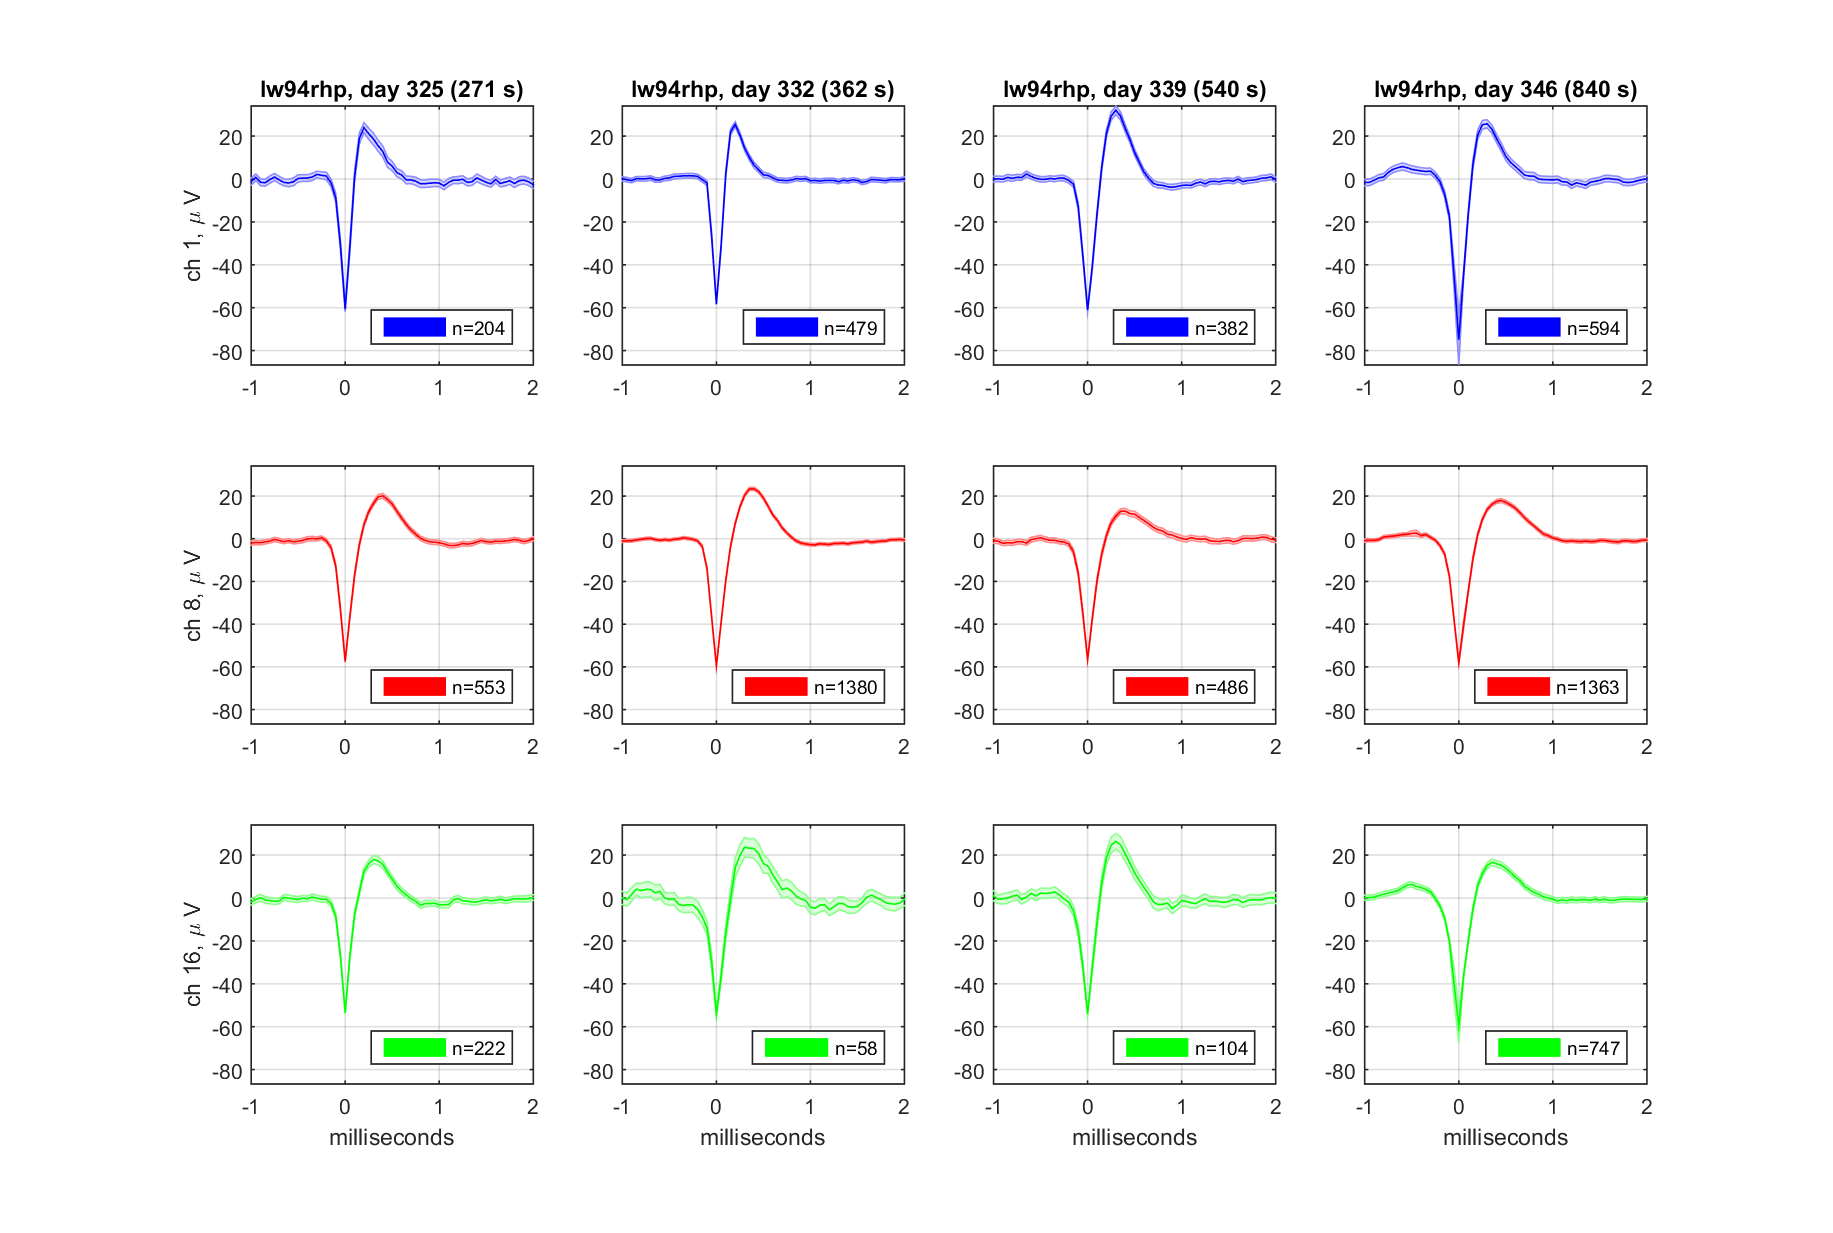
\includegraphics[width=\textwidth]{XSpikeRecording}
  \caption{Some of the electrodes in Area X record spikes after nearly a year.  The column titles show the day post-surgery and the number of seconds of recorded data (for bird lw94rhp).  Each row is one electrode (shown here: only the three best of 16).  Legends show the number of spikes; shaded region is mean $\pm$ 95\% confidence.}
  \label{fig:XSpikeRecording}
\end{figure}


\subsection{Stimulation}

\subsubsection{Minimising stimulation voltage}

\begin{figure}
  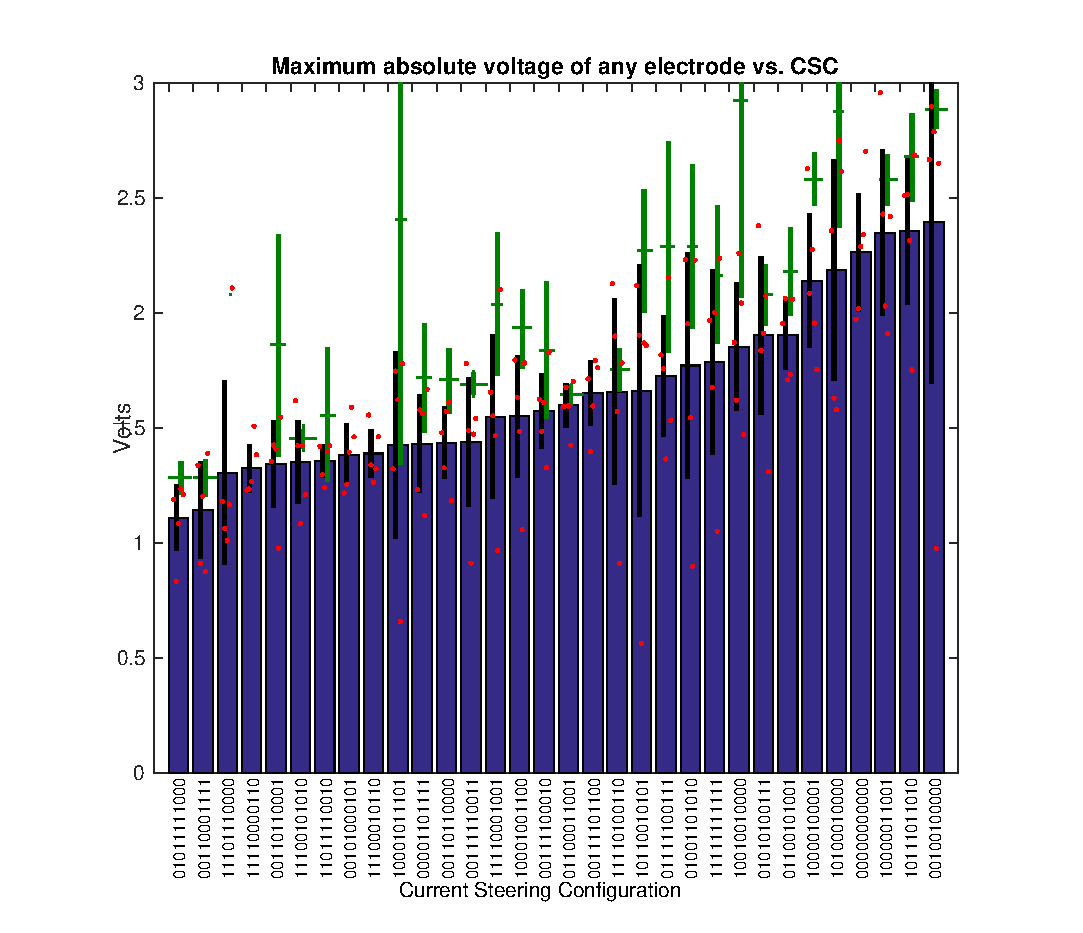
\includegraphics[width=\textwidth]{VoltageVsCSC}
  \caption{The peak X stimulation voltage required in order to achieve biologically effective levels of stimulation in HVC varies with different current-steering configurations.  Here are 32 different configurations, over 5 trials each.  The X axis lists the configuration (each of the 11 active electrodes delivers a positive-first ``0'' or negative-first current-controlled pulse ``1'' pulse).  The Y axis shows the maximum voltage across any electrode.  Error bars are 95\% confidence intervals (n=5), and red dots are the individual trials.  For some CSCs, not all trials evoked a response before our 3V threshold was exceeded, and so the true number is higher.}
  \label{fig:VoltageVsCSC}
\end{figure}

\subsubsection{Controlling the antedromic response}

\begin{figure}
  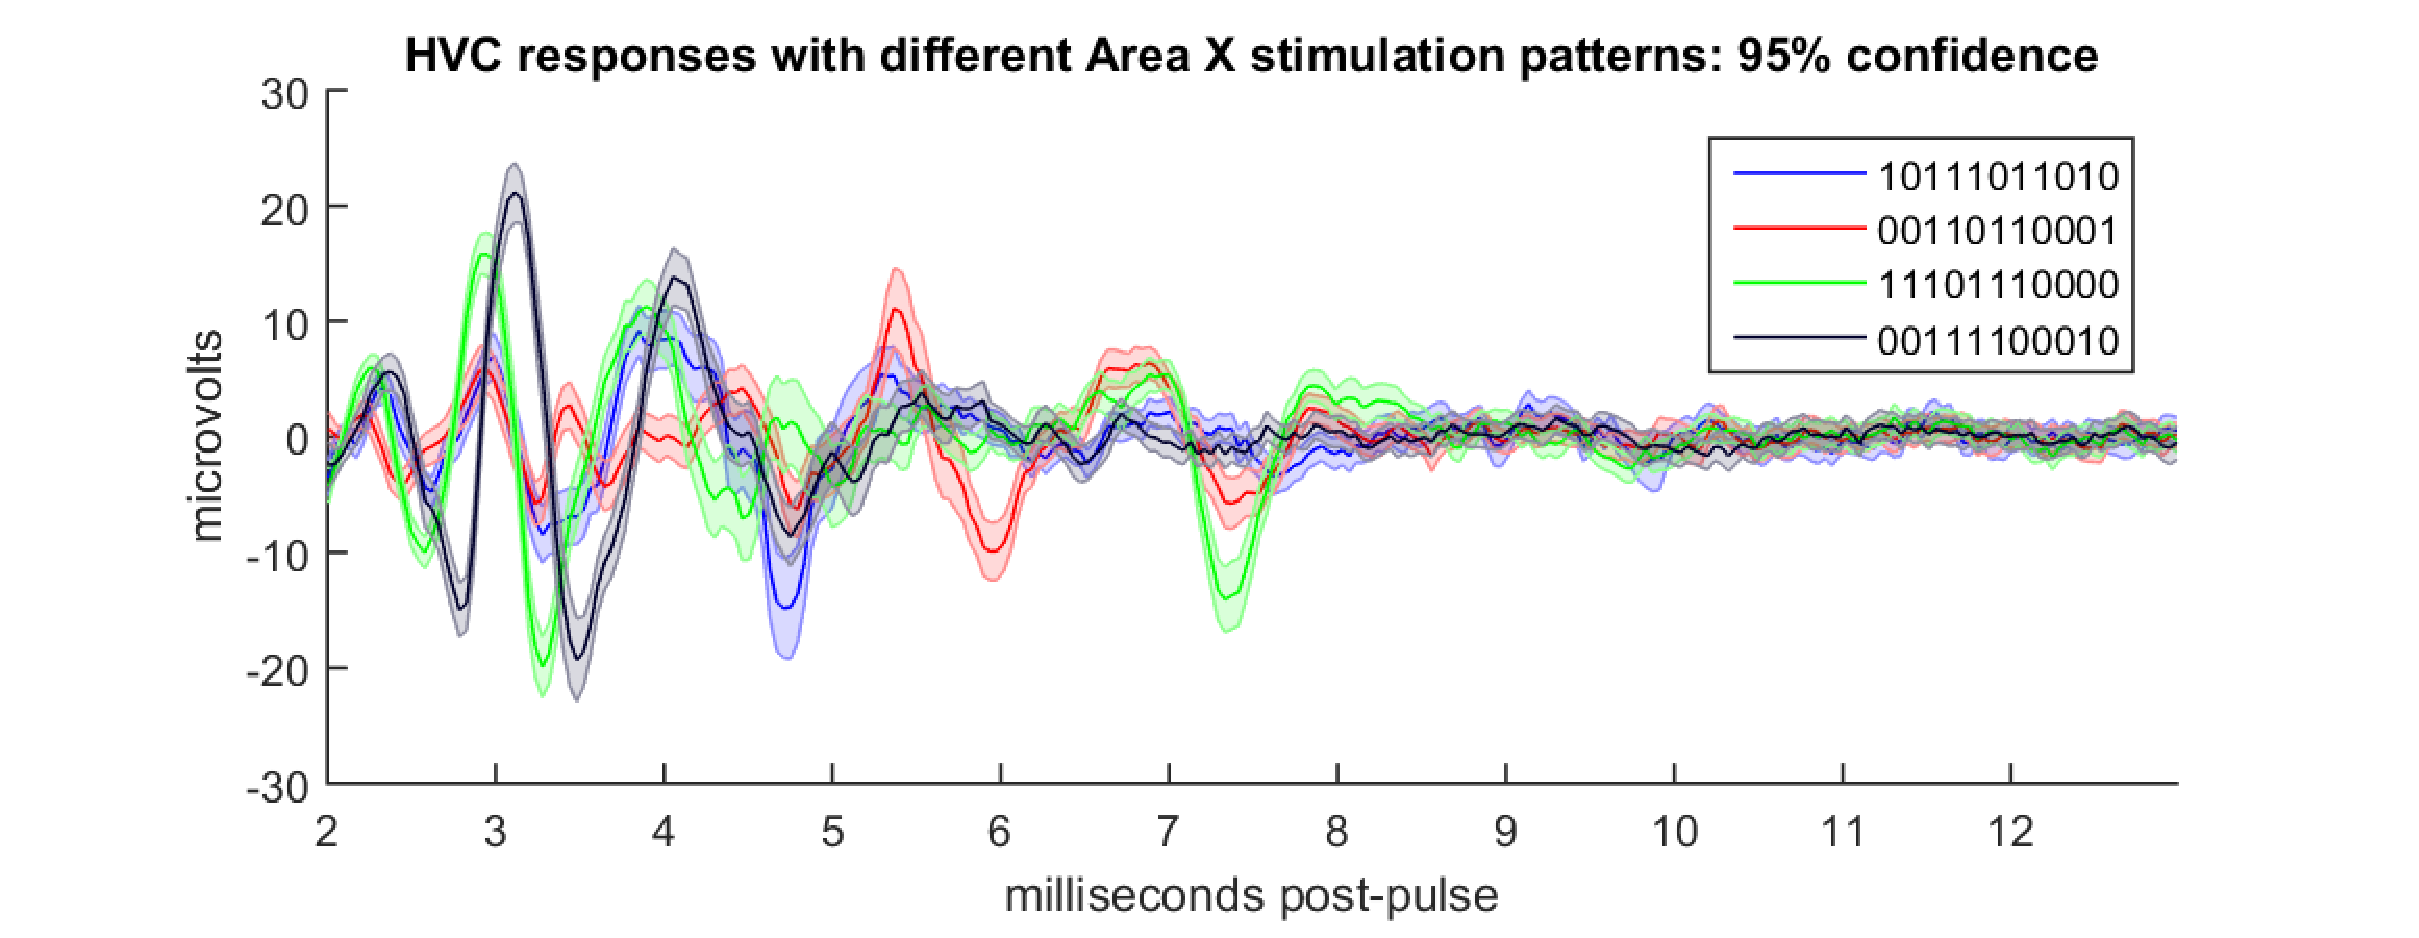
\includegraphics[width=\textwidth]{HVCresponseVsCSC}
  \caption{Different CSCs delivered to Area X can induce different responses antedromically in HVC.  Here are four of the most distinct responses to four of the 32 CSCs shown in \fig{fig:VoltageVsCSC}.  Shading is 95\% confidence, n=198.}
  \label{fig:HVCresponseVsCSC}
\end{figure}


\section{Discussion}

  \cite{Histed2009stimulation}

\bibliography{current}

\end{document}

